\documentclass{article}
\usepackage{fullpage}
\usepackage[utf8]{inputenc}
\usepackage{pict2e}
\usepackage{amsmath}
\usepackage{enumitem}
\usepackage{eurosym}
\usepackage{mathtools}
\usepackage{amssymb, amsfonts, latexsym, cancel}
\setlength{\parskip}{0.3cm}
\usepackage{graphicx}
\usepackage{fontenc}
\usepackage{slashbox}
\usepackage{setspace}
\usepackage{gensymb}
\usepackage{accents}
\usepackage{adjustbox}
\setstretch{1.35}
\usepackage{bold-extra}
\usepackage[document]{ragged2e}
\usepackage{subcaption}
\usepackage{tcolorbox}
\usepackage{xcolor, colortbl}
\usepackage{wrapfig}
\usepackage{empheq}
\usepackage{array}
\usepackage{parskip}
\usepackage{arydshln}
\graphicspath{ {images/} }
\renewcommand*\contentsname{\color{black}Índice} 
\usepackage{array, multirow, multicol}
\definecolor{lightblue}{HTML}{007AFF}
\usepackage{color}
\usepackage{etoolbox}
\usepackage{listings}
\usepackage{mdframed}
\setlength{\parindent}{0pt}
\usepackage{underscore}
\usepackage{hyperref}
\usepackage{tikz}
\usepackage{tikz-cd}
\usetikzlibrary{shapes, positioning, patterns}
\usepackage{tikz-qtree}
\usepackage{biblatex}
\usepackage{pdfpages}
\usepackage{pgfplots}
\usepackage{pgfkeys}
\addbibresource{biblatex-examples.bib}
\usepackage[a4paper, left=1cm, right=1cm, top=1cm,
bottom=1.5cm]{geometry}
\usepackage{titlesec}
\usepackage{titletoc}
\usepackage{tikz-3dplot}
\usepackage{kbordermatrix}
\usetikzlibrary{decorations.pathreplacing}
\newcommand{\Ej}{\textcolor{lightblue}{\underline{Ejemplo}}}
\setlength{\fboxrule}{1.5pt}

% Configura el formato de las secciones utilizando titlesec
\titleformat{\section}
{\color{red}\normalfont\LARGE\bfseries}
{Tema \thesection:}
{10 pt}
{}

% Ajusta el formato de las entradas de la tabla de contenidos
\addtocontents{toc}{\protect\setcounter{tocdepth}{4}}
\addtocontents{toc}{\color{black}}

\titleformat{\subsection}
{\normalfont\Large\bfseries\color{red}}{\thesubsection)}{1em}{\color{lightblue}}

\titleformat{\subsubsection}
{\normalfont\large\bfseries\color{red}}{\thesubsubsection)}{1em}{\color{lightblue}}

\newcommand{\bboxed}[1]{\fcolorbox{lightblue}{lightblue!10}{$#1$}}
\newcommand{\rboxed}[1]{\fcolorbox{red}{red!10}{$#1$}}

\DeclareMathOperator{\N}{\mathbb{N}}
\DeclareMathOperator{\Z}{\mathbb{Z}}
\DeclareMathOperator{\R}{\mathbb{R}}
\DeclareMathOperator{\Q}{\mathbb{Q}}
\DeclareMathOperator{\K}{\mathbb{K}}
\DeclareMathOperator{\im}{\imath}
\DeclareMathOperator{\jm}{\jmath}
\DeclareMathOperator{\col}{\mathrm{Col}}
\DeclareMathOperator{\fil}{\mathrm{Fil}}
\DeclareMathOperator{\rg}{\mathrm{rg}}
\DeclareMathOperator{\nuc}{\mathrm{nuc}}
\DeclareMathOperator{\dimf}{\mathrm{dimFil}}
\DeclareMathOperator{\dimc}{\mathrm{dimCol}}
\DeclareMathOperator{\dimn}{\mathrm{dimnuc}}
\DeclareMathOperator{\dimr}{\mathrm{dimrg}}
\DeclareMathOperator{\dom}{\mathrm{Dom}}
\DeclareMathOperator{\infi}{\int_{-\infty}^{+\infty}}
\newcommand{\dint}[2]{\int_{#1}^{#2}}

\newcommand{\bu}[1]{\textcolor{lightblue}{\underline{#1}}}
\newcommand{\lb}[1]{\textcolor{lightblue}{#1}}
\newcommand{\db}[1]{\textcolor{blue}{#1}}
\newcommand{\rc}[1]{\textcolor{red}{#1}}
\newcommand{\tr}{^\intercal}

\renewcommand{\CancelColor}{\color{lightblue}}

\newcommand{\dx}{\:\mathrm{d}x}
\newcommand{\dt}{\:\mathrm{d}t}
\newcommand{\dy}{\:\mathrm{d}y}
\newcommand{\dz}{\:\mathrm{d}z}
\newcommand{\dth}{\:\mathrm{d}\theta}
\newcommand{\dr}{\:\mathrm{d}\rho}
\newcommand{\du}{\:\mathrm{d}u}
\newcommand{\dv}{\:\mathrm{d}v}
\newcommand{\tozero}[1]{\cancelto{0}{#1}}
\newcommand{\lbb}[2]{\textcolor{lightblue}{\underbracket[1pt]{\textcolor{black}{#1}}_{#2}}}
\newcommand{\dbb}[2]{\textcolor{blue}{\underbracket[1pt]{\textcolor{black}{#1}}_{#2}}}
\newcommand{\rub}[2]{\textcolor{red}{\underbracket[1pt]{\textcolor{black}{#1}}_{#2}}}

\author{Francisco Javier Mercader Martínez}
\date{}
\title{Machine Learning II\\Problemas Tema 1}

\begin{document}
\maketitle
\begin{center}
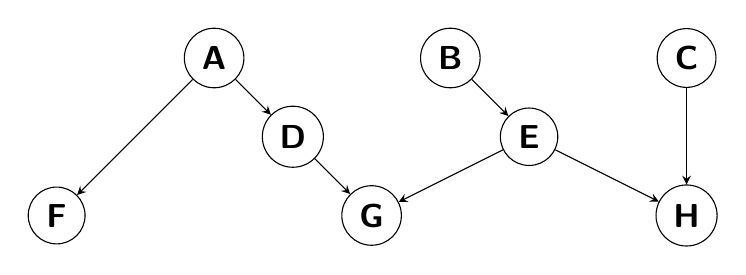
\begin{tikzpicture}[
		state/.style={circle,draw,font=\sffamily\large\bfseries},
		>=stealth
		]
        \node[state] (A) at (0,0) {A};
        \node[state] (B) at (3,0) {B};
        \node[state] (C) at (6,0) {C};
        \node[state] (D) at (1,-1) {D};
        \node[state] (E) at (4,-1) {E};
        \node[state] (F) at (-2,-2) {F};
        \node[state] (G) at (2,-2) {G};
        \node[state] (H) at (6,-2) {H};
    
        \draw[->] (A) -- (D);
        \draw[->] (A) -- (F);
        \draw[->] (D) -- (G);
        \draw[->] (B) -- (E);
        \draw[->] (E) -- (G);
        \draw[->] (E) -- (H);
        \draw[->] (C) -- (H);
\end{tikzpicture}
\end{center}
\begin{itemize}[label=\textbullet]
    \item Nodo A:
        \begin{itemize}[label=\textbullet]
            \item Independiente de B, C, H, E
            \item Dado D, F: independiente de B, E, C, H, G
        \end{itemize}
    \item Nodo G:
        \begin{itemize}[label=\textbullet]
            \item Dados D, E: independiente de A, F, B, C, H
        \end{itemize}
    \item Nodo E:
        \begin{itemize}[label=\textbullet]
            \item Dado B: independiente de A, D, F, C
            \item Dados B, G, H, D, C: independiente de A, F
        \end{itemize}
\end{itemize}
\vspace{1em}
\hline
\begin{center}
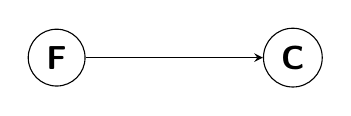
\begin{tikzpicture}[
		state/.style={circle,draw,font=\sffamily\large\bfseries},
		>=stealth
		]
        \node[state] (F) at (0,0) {F};
        \node[state] (C) at (3,0) {C};
        \draw[->] (F) -- (C);
\end{tikzpicture}
\end{center}
$\begin{array}{l}
    P(F)=0.1\to P(\neg F)=0.9\\
    P(C|F)=0.8\to P(\neg C|F)=0.2\\
    P(C|\neg F)=0.3\to P(\neg C|\neg F)=0.7\\
    \text{¿}P(F|C)?
\end{array}$
\[
P(F|C)=\dfrac{P(F,C)}{P(C)}=\dfrac{0.08}{0.35}=0.2286
\] 
$P(F,C)=P(F)\cdot P(C|F)=0.1\cdot 0.8=0.08$

$P(C)=\sum_{f} P(F,C)=\lbb{P(F,C)}{0.08} +P(\neg F,C)=0.35 $ 

$P(\neg F,C)=P(\neg F)\cdot P(C|\neg F)=0.9\cdot 0.3=0.27$

\vspace{1em}
\hline

\begin{center}
    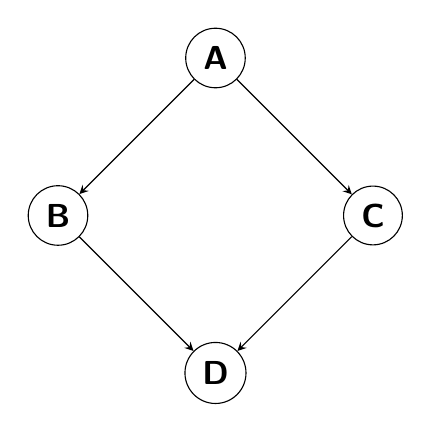
\begin{tikzpicture}[
		state/.style={circle,draw,font=\sffamily\large\bfseries},
		>=stealth
		]
        \node[state] (A) at (0,0) {A}; 
        \node[state] (B) at (-2,-2) {B}; 
        \node[state] (C) at (2,-2) {C}; 
        \node[state] (D) at (0,-4) {D}; 
        
        \draw[->] (A) -- (B);
        \draw[->] (A) -- (C);
        \draw[->] (B) -- (D);
        \draw[->] (C) -- (D);
    \end{tikzpicture}
\end{center}
$\begin{array}{ll}
    P(A)=0.75 & P(\neg A)=0.25\\
    P(B|A)=0.2 & P(\neg B|A)=0.8\\
    P(B|\neg A)=0.5 & P(\neg B|\neg A)=0.5\\
    P(C|A)=0.7 & P(\neg C|A)=0.3\\
    P(C|\neg A)=0.25 & P(\neg C|\neg A)=0.75\\
    P(D|B,C)=0.3 & P(\neg D|B,C)=0.7\\
    P(D|\neg B, C)=0.1 & P(\neg D|\neg B,C)=0.9\\
    P(D|B,\neg C)=0.25 & P(\neg D|B,\neg C)=0.75\\
    P(D|\neg B, \neg C)=0.35 & P(\neg D|\neg B,\neg C)=0.65
\end{array}$

$\begin{array}{l}
    P(A,B,C,D)=P(A)P(B|A)P(C|A)P(D|B,C)\\
    P(A,D)=\sum_b\sum_c P(A,B,C,D)=\sum_b\sum_c P(A)P(B|A)P(C|A)P(D|B,C)\\
    \begin{aligned}
        P(D|A)=\sum_b\sum_cP(B|A)P(C|A)P(D|B,C)&=\sum_b P(B|A)\lbb{\sum_c P(C|A)P(D|B,C)}{f_c(A,B,D)}\\
        &= \sum_bP(B|A)f_c(A,B,D) \\
        &= P(B|A)f_c(A,B,D)+P(\neg B|A)f_c(A,\neg B,D) \\
        &= 0.197 \\
    \end{aligned}\\
    f_c(A,B,D)=P(C|A)P(D|B,C)+P(\neg C|A)P(D|B,\neg C)=0.285\\
    f_c(A,\neg B,D)=P(C|A)P(D|\neg B,C)+P(\neg C|A)P(D|\neg B,\neg C)=0.175\\
\end{array}$
\end{document}
